\subsection{Maurer's universal statistical test}
Maurer's universal test is one of the tests included in NIST SP 800-22 \cite{rukhin2001statistical,bassham2010sp}.
% A statistical test for the randomness of a binary sequence has been proposed by Maurer \cite{maurer1992universal}, and it is included in NIST SP 800-22 \cite{rukhin2001statistical,bassham2010sp}. 
Maurer's universal statistical test aims at detecting non-randomness based on the test statistic value which is relating to the source's entropy, and the non-randomness is evaluated whether the computed entropy attains the maximum or not. 
%
% Unlike the other types of statistical tests which is designed to detect specific defects, Maurer's universal test is able to detect the wide range of statistical defects consists of that those can be modeled by an ergodic stationary source with finite memory. 
Unlike other types of statistical tests which is designed to detect specific defects, Maurer's universal test is able to detect a wide range of statistical defects.
%
%ergodic statistical sourceから生成された系列というのは,各ビットがある確率に従って生成される.その確率は,前に出力されたビット列から決まる.もし,理想的な乱数の場合,前の系列が何であれ,それぞれ1/2の確率で0と1が生成される.
\par
Let us consider an information source $S$ which generates a sequence $U_1,U_2,\dots$. For each $i$, we regard $U_i$ as a sample from a random variable.
 % of random variables. 
A source $S$ is called a finite memory source if there exists a positive integer $M$ such that the conditional probability of $U_n$, given $U_1,\dots,U_{n-1}$, depends only on the most previous $M$ bits, i.e.,
\begin{align}\label{eq:memory}
	P_{U_n\mid U_{n-1}\dots U_{1}}(u_n \mid u_{n-1}\dots u_{1}) = P_{U_n\mid U_{n-1}\dots U_{n-M}}(u_n \mid u_{n-1}\dots u_{n-M}),
\end{align}
for $n>M$ and for every binary sequence $u_1,\dots,u_n\in\{0,1\}^n$. The smallest $M$ satisfying Eq. (\ref{eq:memory}) is called the memory of the source. The probability distribution of $U_n$ is thus determined by the source's state $\Lambda_n = U_{n-M},\dots,U_{n-1}$ at time $n$. Let $\Lambda_1 = U_0 \dots U_{-M+1}$ be the initial state where $U_{-M+1}\dots U_0$ are dummy random variables. Then, the source is called \textit{stationary}, if the information source $S$ satisfies the following relation in addition to Eq. (\ref{eq:memory}),
\begin{align}
	P_{U_n\mid\Lambda_n}(u\mid \lambda) = P_{U_1\mid\Lambda_1}(u\mid \lambda),
\end{align}
for all $n>M$, $u\in\{0,1\}$ and $\lambda \in \{0,1\}^M$. 
%
% Therefore, the probability of taking each bit to be ``$1$'' or ``$0$'' is given by a probability and it depends only on the most previous finite sequence when a sequence is generated by a stationary source. 
%
Therefore, it depends only on the most previous $M$-bit sequence when a sequence is generated by a stationary source.
%
On the other hand, each bit is independent of the previous sequence, and the probability of taking ``$1$'' or ``$0$'' is exactly the same as $\frac{1}{2}$ if we say a sequence is truly random in intuitive sense.
%
% For a binary sequence generated by an ergodic stationary source, each bit takes ``$1$'' or ``$0$'' in some probability. The probability of taking $n$-th bit to be ``$1$'' or ``$0$'' is depend only on the most previous bits, that is, the following relation holds.
% \begin{align}
% 	P_{U_n\mid U_{n-1}\dots U_{1}}(u_n \mid u_{n-1}\dots u_{1}) = P_{U_n\mid U_{n-1}\dots U_{n-M}}(u_n \mid u_{n-1}\dots u_{n-M}),
% \end{align}
% where $M$ is called memory of the source. For a truly random sequence, the probability of taking each bit to be $1$ or $0$ is independent of previous bits, and the probability of taking each bit to be $1$ or $0$ is exactly the same as $\frac{1}{2}$. 
% any one of the general class of statistical defects which can be modeled by ergodic stationary source with finite memory. 
%
\par
%
The formulation of Maurer's universal test is motivated by the universal source coding algorithms that has been proposed in \cite{elias1987interval,willems1989universal} and the procedure is described as follows. In the following, let $B$ be the set $\{0,1\}$, and $x^n = x_1,x_2,\dots,x_n \in B^n$ be a binary sequence of length $n$, where $x_i\in B$. The test takes as input three positive integers $L,\,Q$ and $K$, and a binary sequence $s^n \in B^n$ generated by a tested source. The sequence is divided into adjacent non-overlapping blocks of length $L$. Then, the first $Q$ blocks ($L\times Q$-bits) are used for initialization, and the remaining $K$ blocks ($L\times K$-bits) are used for the test. Without loss of generality, we can assume that $n=L\times(Q+K)$ holds\footnote{%
If the relation $n=L\times(Q+K)$ does not hold, then let $K$ be $\left\lfloor \frac{n}{L} \right\rfloor - Q$.
}. 
%
Let $b_k(x^n)$ be the $k$-th block of $x^n$, i.e., $b_k(x^n) = x_{L(k-1)+1}, x_{L(k-1)+2}, \dots, x_{Lk}$. Considering the situation that the $(n-m)$-th block takes the same value with the $n$-th block and the blocks from $(n-m+1)$-th to $(n-1)$-th blocks do not take the value, we define an integer-valued variable $A_n(x^n)$ as $m$. 
% The mapping from a binary sequence $x^n$ to a integer-valued variable $A_n(x^n)$ is given by
% \begin{align}
% 	A_{n}(x^n) = \left\{ \begin{array}{ll}
% 	n, \:\: &\text{if} \:\: b_{n-m} \neq b_n \:\: \text{for} \:\: 1 \leq m \leq n-1, \\
% 	\min \{ m\in\mathbb{N} \mid m \geq 1, b_{n-m} = b_n \}, \:\: &\text{otherwise}.
% 	\end{array} \right.
% \end{align}
% for $n=Q+1,Q+2,\dots,Q+K$.
%
Figure \ref{fig:A_n_example} illustrates an example for $L=3$. The test function $f_M$, which maps a binary sequence to a real number, is defined by 
% The test statistic value $f_M:B^{n} \to \mathbb{R}$ is defined as the average of the binary logarithm of $A_{Q+1},A_{Q+2},\dots,A_{Q+K}$, i.e., 
\begin{align}\label{eq:fM}
	f_M(x^n) = \frac{1}{K} \sum_{n=Q+1}^{Q+K} \log_2 A_n(x^n),
\end{align}
where $A_n(x^n)$ is defined by
\begin{align}\label{eq:An}
	A_{n}(x^n) = \left\{ \begin{array}{ll}
	n, \quad \text{if} \:\: b_{n-m}(x^n) \neq b_n(x^n) \:\: \text{for} \:\: 1 \leq m \leq n-1, \\
	\min \{ m\in\mathbb{N} \mid m \geq 1,\, b_{n-m}(x^n) = b_n(x^n) \}, \quad \text{otherwise},
	\end{array} \right.
\end{align}
for $n=Q+1,Q+2,\dots,Q+K$.
% The mapping from $f_M(x^n)$ to the p-value $p_M$ is given by
% \begin{align}
% 	% p\mathchar`- \mathrm{value}_M 
% 	p_M
% 	= \mathrm{erfc} \left( \left| \frac{f_M(x^n) - \mathbb{E}[f_M(R^n)]}{\sqrt{2} \sigma_M} \right| \right),
% \end{align}
% where $R^n$ denotes a binary sequence of length $n$ generated by a BSS.
% where $\mathbb{E}[f_M(R^n)]$ denotes the expectation value, $\sigma_M^2$ denotes the variance of $f_M(R^n)$ under null hypothesis, and the $\mathrm{erfc}$ is the complementary error function defined by
% \begin{align}
%    \text{erfc}(z) = \frac{2}{\sqrt{\pi}} \int_{z}^{\infty} \mathrm{e}^{-t^2}\, \mathrm{d}t.
% \end{align}
%-------------------------------------------------------------------
\begin{figure}
\centering
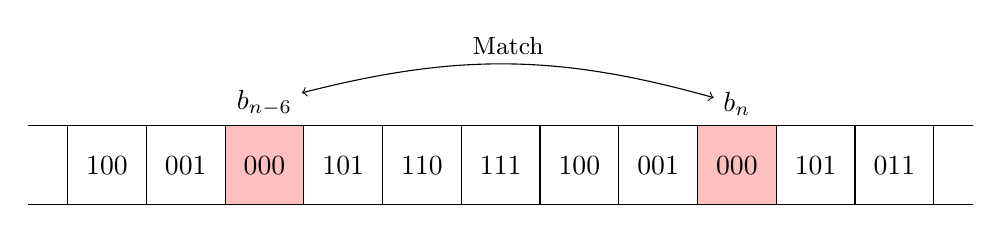
\begin{tikzpicture}
\draw (-1.5,0)--(-1.0,0);
\draw (-1.5,1)--(-1.0,1);
\draw (-1.0,0) rectangle (0,1) node at (-0.5, 0.25) [above] {$100$};
\draw (0,0) rectangle (1,1) node at (0.5, 0.25) [above] {$001$};
\filldraw [draw=black, fill=pink] (1,0) rectangle (2,1) node at (1.5, 0.25) [above] {$000$} node (A) at (1.5, 1.0) [above] {$b_{n-6}$};
\filldraw [draw=black, fill=white] (2,0) rectangle (3,1) node at (2.5, 0.25) [above] {$101$} ;
\filldraw [draw=black, fill=white] (3,0) rectangle (4,1) node at (3.5, 0.25) [above] {$110$};
\filldraw [draw=black, fill=white] (4,0) rectangle (5,1) node at (4.5, 0.25) [above] {$111$};
\filldraw [draw=black, fill=white] (5,0) rectangle (6,1) node at (5.5, 0.25) [above] {$100$};
\filldraw [draw=black, fill=white] (6,0) rectangle (7,1) node at (6.5, 0.25) [above] {$001$};
\filldraw [draw=black, fill=pink] (7,0) rectangle (8,1) node at (7.5, 0.25) [above] {$000$} node (AA) at (7.5, 1.0) [above] {$b_n$};
\draw (8,0) rectangle (9,1) node at (8.5, 0.25) [above] {$101$};
\draw (9,0) rectangle (10,1) node at (9.5, 0.25) [above] {$011$};
\draw (10,0)--(10.5,0);
\draw (10,1)--(10.5,1);
%
\draw[<->] (A) to[bend left=15] node [above] {\small Match} (AA);
\end{tikzpicture}
\caption{An example of the situation of $A_n=6$ for $L=3$.}
\label{fig:A_n_example}
\end{figure}
%-------------------------------------------------------------------
%
\par
%
In order to evaluate the non-randomness of a given binary sequence, it is necessary to derive the expected value and the variance of the reference distribution for a truly random sequence. Note that a truly random sequence is a binary sequence generated by a uniform distribution on $\{0,1\}^n$. 
% It has been shown in \cite{maurer1992universal} that the following relations hold under admissible assumption $Q\to\infty$.
Under the assumption $Q\to\infty$, the expectation and the variance are given by
% a binary sequence of length $n$ generated by a binary symmetric source (BSS) which means a truly random sequence. Let $R^n$ be a binary random sequence of length $n$ generated by a BSS. It has been show in \cite{maurer1992universal} that $\mathbb{E}[f_M(R^n)]$ and $\sigma_M^2$ are obtained as
\begin{align}
	\mathbb{E}[f_M(R^n)]  &= 2^{-L}\sum_{i=1}^{\infty}(1-2^{-L})^{i-1} \log_2 i \label{eq:mean_maurer},\\
	\sigma_M^2 &= c_M(L,K)^2 \times \frac{\mathrm{Var}[\log_2 A_n(R^n)]}{K} \label{eq:sigma_maurer},
\end{align}
%
where $R^n$ denotes a truly random sequence of length $n$. 
% represents the correction factor by which $\sigma_M^2$ is reduced compared with what it would be if the terms $A_n(R^n)$ were independent. It has been proposed in \cite{maurer1992universal} that $c_M(L,K)$ for $K\geq 2^L$ can be approximated by
%
In \cite{maurer1992universal}, the following approximation is empirically proposed:
% It is necessary to derive the expected value $\mathbb{E}[f_M(R^n)]$ and the variance $\sigma_M^2$ for calculating p-value from Eq. (). It is shown in \cite{maurer1992universal} that $\mathbb{E}[f_M(R^n)]$ and $\sigma_M^2$ are obtained as
% \begin{align}
% 	\mathbb{E}[f_M(R^n)] &= \mathbb{E}[\log_2 A_n] = 2^{-L}\sum_{i=1}^{\infty}(1-2^{-L})^{i-1} \log_2 i,\\
% 	\sigma_M^2 &= \mathrm{Var}[f_M(R^n)] = c_M(L,K)^2 \times \frac{\mathrm{Var}[\log_2 A_n]}{K},
% \end{align}
% where $c_M(L,K)$ is the correction factor by which $\sigma_M^2$ is reduced compared with what it would be if the terms $A_n$ were independent. It is suggested in \cite{maurer1992universal} that $c_M(L,K)$ can be approximated as
\begin{align}\label{eq:cM_maurer}
	c_M(L,K) \simeq 0.7 - \frac{0.8}{L} + \left( 1.6 + \frac{12.8}{L} \right) K^{-4/L}.
\end{align}
The approximation above has been obtained by numerical simulations. 
%
In \cite{coron1998accurate}, the accurate expression of $c_M(L,K)$ has been obtained theoretically. 
% However, it has a high computational cost that an approximated value $c_M(L,K)$ for $K\geq33\times2^L$ is given as follows:
However, it requires much cost to compute the $c_M(L,K)$ for given $L$ and $K$, and hence an approximation of the theoretical form is given as follows:

% by deriving the joint distribution of $(A_n(R^n),\,A_{n+k}(R^n))$
 % and $c_M(L,K)$ for $K\geq33\times2^L$ is shown to be approximated by
% It also has been suggested in \cite{coron1998accurate} that the precise value of $c_M(L,K)$ for $K\geq33\times2^L$ is expressed as
\begin{align}\label{eq:cM_coron}
	c_M(L,K)^2 \simeq d_M(L) + \frac{e_M(L)\times2^L}{K}, 
\end{align} 
where $d_M(L)$ and $e_M(L)$ are listed in \cite{coron1998accurate} for $L=3,4,\dots,16$. 
The approximation in Eq. (\ref{eq:cM_coron}) is accurate for $K\geq 33\times 2^L$ in practice.
%
Note that $\mathrm{Var}[\log_2 A_n]$ in Eq. (\ref{eq:sigma_maurer}) can be computed by the definition of variance by
\begin{align}
 	\mathrm{Var}[\log_2 A_n(R^n)] = 2^{-L}\sum_{i=1}^{\infty}(1-2^{-L})^{i-1} (\log_2 i)^2 - (\mathbb{E}[f_M(R^n)])^2.
\end{align}
% where $\mathbb{E}[f_M(R^n)]$ is given by Eq. (\ref{eq:mean_maurer}).
% the values are listed in \cite{maurer1992universal} for $L=1,2,\dots,16$.
%
\par
%
To implement the test, it is necessary to set the parameters. In \cite{maurer1992universal}, the study recommends to set parameters $L\,Q$ and $K$ as $6\leq L,\, \leq 16$, $Q \geq 10 \times 2^L$ and $K \geq 1000\times 2^L$, respectively. 
%
The study also insists that rejection rate $\rho$ should be chosen as $\rho \in [0.001, 0.01]$. 
%
Then, it is concluded that the null hypothesis of Maurer's test\footnote{A null hypothesis of Maurer's test is that a binary sequence of length $n$ follows a uniform distribution on $\{0,1\}^n$} 
is rejected if either $f_M(x^n)<t_1$ or $f_M(x^n)>t_2$ holds, where the thresholds $t_1$ and $t_2$ are written as
\begin{align}\label{eq:ysigma}
\begin{split}
	t_1 &= \mathbb{E}[f_M(R^n)] - y\sigma_M, \\
	t_2 &= \mathbb{E}[f_M(R^n)] + y\sigma_M.
\end{split}
\end{align}
Using the complementary error function $\mathrm{erfc}$ defined by
\begin{align}
   \text{erfc}(z) = \frac{2}{\sqrt{\pi}} \int_{z}^{\infty} \mathrm{e}^{-u^2} \, \mathrm{d}u,
\end{align}
the value $y$ in Eq. (\ref{eq:ysigma}) is given as $\mathrm{erfc}(y)=\frac{\rho}{2}$. 
% where $\mathrm{erfc}(y)=\frac{\rho}{2}$. Note that $\mathrm{erfc}$ is the complementary error function defined by
% \begin{align}
%    \text{erfc}(z) = \frac{2}{\sqrt{\pi}} \int_{z}^{\infty} \mathrm{e}^{-u^2} \, \mathrm{d}u.
% \end{align}
% In the above relation, the standard deviation $\sigma_M$ is given by Eqs. (\ref{eq:sigma_maurer}) or (\ref{eq:cM_coron}) and $y$ is the number of standard deviations that the computed test statistic value $f_M(x^n)$ is allowed to be away from the expected value $\mathbb{E}[f_M(R^n)]$. The parameter $y$ should be chosen such that $\mathcal{N}(-y)=\frac{\rho}{2}$ where $\mathcal{N}:\mathbb{R}\to\mathbb{R}$ is the integral of the normal density function defined by
% Note that $y$ in the above equation satisfies
% \begin{align}
% 	\frac{1}{\sqrt{2\pi}}\int_{-\infty}^{-y} \mathrm{e}^{-\frac{u^2}{2}} \, \mathrm{d}{u} = \frac{\rho}{2}.
% \end{align}
Notice that it is implicitly assumed that $f_M(R^n)$ follows a normal distribution.
%
\par
In NIST SP 800-22, the non-randomness is evaluated by the p-value shown as
\begin{align}
	p\mathchar`- \mathrm{value}_M 
	% p_M
	= \mathrm{erfc} \left( \left| \frac{f_M(x^n) - \mathbb{E}[f_M(R^n)]}{\sqrt{2} \sigma_M} \right| \right),
\end{align}
where $\mathrm{erfc}$ is the complementary error function defined by
% \begin{align}
%    \text{erfc}(z) = \frac{2}{\sqrt{\pi}} \int_{z}^{\infty} \mathrm{e}^{-u^2} \, \mathrm{d}u.
% \end{align}
Then, the null hypothesis of Maurer's test is rejected if $p\mathchar`- \mathrm{value}_M < \alpha$, where $\alpha$ is a significance level.
%
% In NIST SP 800-22 \cite{rukhin2001statistical,bassham2010sp}, the non-randomness of a given binary sequence $x^n\inB^n$ is evaluated by the p-value defined by
% % the mapping from $f_M(x^n)$ to the p-value is given by
% \begin{align}
% 	p\mathchar`- \mathrm{value}_M 
% 	% p_M
% 	= \mathrm{erfc} \left( \left| \frac{f_M(x^n) - \mathbb{E}[f_M(R^n)]}{\sqrt{2} \sigma_M} \right| \right),
% \end{align}
% where $\mathrm{erfc}$ is the complementary error function defined by
% \begin{align}
%    \text{erfc}(z) = \frac{2}{\sqrt{\pi}} \int_{z}^{\infty} \mathrm{e}^{-u^2} \, \mathrm{d}u.
% \end{align}
% %
% In the case that the computed p-value is less than the significance level $\alpha$, it is concluded that a binary sequence being tested is not random. 
%-------------------------------------------------------------------
%-------------------------------------------------------------------
%-------------------------------------------------------------------
\par
There is much concern in the asymptotic relation between the Maurer's test statistic and the source's per-bit entropy. In \cite{maurer1992universal}, the expected value of the test statistic for a truly random sequence $\mathbb{E}[f_M(R^n)]$ is closely related to the entropy of blocks. It has been shown that the following relation holds:
\begin{align}\label{eq:maurer_asymptotic_R}
	\lim_{L\to\infty} \left[ \mathbb{E}[f_M(R^n)] -L \right] = C,
\end{align}
where $C$ is a constant whose value is equal to $-\frac{\ln 2}{\gamma} \simeq -0.8327$ and $\gamma$ is Euler's constant \cite{hardy1979introduction}. We provide the proof of $C=-\frac{\ln 2}{\gamma}$ is given in Appendix \ref{appendix:A}. 
%
Let us consider a binary sequence $U_{\mathrm{BMS}_p}^n$ generated by a binary memoryless source $\mathrm{BMS}_p$. Note that a sequence $U_{\mathrm{BMS}_p}^n$ follows a distribution on $\{0,1\}^n$ taking each bit to be ``$1$'' with probability $p\in (0,1)$ independently. 
% We can show that the relation $K_L=L\times H(p)$ holds for a binary memoryless source.
%
For a binary sequence $U_{\mathrm{BMS}_p}^n \in B^n$, the following relation
\begin{align}
	\lim_{L\to\infty} \left[ \mathbb{E}[f_M(U_{\mathrm{BMS}_p}^n)] -L\times H(p) \right] = C
\end{align}
holds for any $p \in (0,1)$, where $H$ is the binary entropy function corresponding to $\mathrm{Pr}[X=1]=p$. Here, $X$ is a random variable. 
%
In \cite{maurer1992universal}, a similar result has been studied to show for a binary sequence $U_s^n$ generated by every ergodic stationary source $S$. The study in \cite{coron1998accurate} develops the idea and proves that the following relation holds:
% It has been conjectured in \cite{maurer1992universal} that the similar result would hold for every binary ergodic stationary source $S$ with output sequence $U_s^n$,
\begin{align}
	\lim_{L\to\infty} \left[ \mathbb{E}[f_M(U_s^n)] - K_L \right] = C,
\end{align}
where $K_L$ is equivalent to the entropy of $L$ bit blocks defined by
\begin{align}\label{eq:K_L}
	K_L = -\sum_{b \in B^n} \mathrm{Pr}[b] \log_2 \mathrm{Pr}[b].
\end{align}
Other asymptotic relations between Maurer's test statistic and a source's entropy can be found in \cite{wegenkittl2001entropy,choe2000average,abadi2004version,kim2014estimation,kim2018low}.
% It has been proven in \cite{coron1999security} that test statistic given in Eq. (\ref{eq:fM}) is closely related to the source's entropy.
% % The test statistic is closely related to the source's per-bit entropy.
% It has been proven in \cite{maurer1992universal} that the following relation holds for a binary binary symmetric source generated by STP.
% \begin{align}
% 	\lim_{L\to\infty} \left[ \mathbb{E}[f_M(R^n)] -L \right] = C = -\frac{\ln 2}{\gamma}.
% \end{align}
% where $C$ is a constant whose value is proven to be equal to $-\frac{\ln 2}{\gamma}$. The proof is given in Appendix.
% It has been conjectured that the same relation holds for any binary ergodic stationary source $U_s^n$.
% \begin{align}
% 	\lim_{L\to\infty} \left[ \mathbb{E}[f_M(U_s^n)] -L\times H(q) \right] = C.
% \end{align}
% However, it has been in \cite{coron1998accurate} proven that the above relation does not hold, and refuse that.
% \begin{align}
% 	\lim_{L\to\infty} \left[ \mathbb{E}[f_M(U_s^n)] - H_s \right] = C.
% \end{align}
% where $H_s$ is the entropy.
%-------------------------------------------------------------------
%-------------------------------------------------------------------
% \par
% It has proven in \cite{maurer1992universal} that $\mathbb{E}[f_M(R^n)]-L$ converges to the constant $C=-0.832746$ as $L\to\infty$, and conjectured that the following relation holds for any $q\in (0,1)$. 
% \begin{align}
% 	\lim_{L\to\infty} \left[ \mathbb{E}[f_M(U_S^n)] - L\times H(q) \right] = C.
% \end{align}
% However, it has proven in \cite{coron1999security} that the conjecture does not correct in the case of $q \neq 0.5$.
%-------------------------------------------------------------------%
%-------------------------------------------------------------------%
% \begin{algorithm}[t]
% \caption{The procedure of Maurer's universal statistical test based on NIST SP 800-22}
% % \label{alg:1}
% \begin{algorithmic}[1]
% \State Set the positive integers $L,\, Q$ and $K$ as a parameter, a significance level $\alpha$, and the number of sample sequences $m$.
% \State Divide a binary sequence $x^n$ into adjacent non-overlapping blocks of length $L$, and compute $A_n$ for $n=Q+1,Q+2,\dots,Q+K$ from Eq.(\ref{eq:An}). \label{state:divide}
% % The recommendation is $L$ as between $6$ and $16$, $Q \geq 10\times2^L$, $K \geq 1000\times2^L$. 
% % \State Divide a binary sequence $x^n$ into adjacent non-overlapping blocks of length $L$ and calculate $A_n$ from Eq. (\ref{eq:An}) for $n=Q+1,Q+2,\dots,Q+K$.
% \State Compute a test statistic from Eq.(\ref{eq:fM}).
% \State Compute a $p \, \mathchar`- \mathrm{value}$ from Eq. (\ref{eq:pM}). \label{state:pvalue}
% % \State If the computed p-value is less than $\alpha$, then conclude the sequence is non-random. Otherwise, conclude the sequence is random.
% \State Do \ref{state:divide} to \ref{state:pvalue} for $m$ sample sequences, and obtain $m$ p-values.
% \State (Second-level test Ⅰ: Proportion of sequences passing a test)
% \State (Second-level test Ⅰ: Proportion of sequences passing a test)
% \end{algorithmic}
% \end{algorithm}
%-------------------------------------------------------------------%
%-------------------------------------------------------------------%
%-------------------------------------------------------------------%
%-------------------------------------------------------------------%
%-------------------------------------------------------------------%
%-------------------------------------------------------------------%
%-------------------------------------------------------------------%
%-------------------------------------------------------------------%
%-------------------------------------------------------------------%
%-------------------------------------------------------------------%
%-------------------------------------------------------------------%
%-------------------------------------------------------------------%
%-------------------------------------------------------------------%
%-------------------------------------------------------------------%
%-------------------------------------------------------------------%
\subsection{Coron's universal statistical test}
As seen in the previous subsection, Maurer's universal test can detect a wide range of statistic defects modeled by an ergodic statistic source with finite memory, however, the test only provides an asymptotic measure of the source's entropy. 
%
To address the problem, a modified version of Maurer's universal test called ``Coron's universal test'' has been proposed in \cite{coron1999security}. In this test, the expectation of test statistic value is exactly equal to the source's entropy. The main procedure is the same as Maurer's test except for the test statistic. The test function $f_C$, which maps a binary sequence to a real number, is defined by 
% The test function $f_C:B^n\to\mathbb{R}$ is defined as
\begin{align}\label{eq:fC}
	f_C(x^n) = \frac{1}{K} \sum_{n=Q+1}^{Q+K} g(A_n(x^n)),
\end{align}
where $A_n(x^n)$ is defined by Eq. (\ref{eq:An}) and $g:\mathbb{N}\to\mathbb{R}$ is given by
% the function $g:\mathbb{N}\to\mathbb{R}$ is defined as
\begin{align}\label{eq:function_g}
	g(m) = (\log_2 \mathrm{e}) \sum_{k=1}^{m-1}\frac{1}{k},
\end{align}
for $m\geq 2$. Note that we set $g(1)=0$.
%
For a binary sequence $U_s^n$ generated by an ergodic stationary source $S$, the expected value is exactly equal to the entropy of $L$ blocks of $S$, i.e.,
\begin{align}\label{eq:coron_expected_value_for_U}
	\mathbb{E}[f_C(U_s^n)] = K_L,
\end{align}
where $K_L$ corresponds to the entropy of blocks given by Eq. (\ref{eq:K_L}).
%
\par
It is necessary to derive the expected value and the variance of the reference distribution just like Maurer's test. From Eq. (\ref{eq:coron_expected_value_for_U}), the expected value for $R^n$ is obtained by
\begin{align}
\label{eq:coron_expected_value_truly_random}
	\mathbb{E}[f_C(R^n)] &= L, 
\end{align}
since $K_L=L$ when the source is the binary symmetric source. 
% It has been obtained \cite{coron1999security} that the variance can be given by
The variance is also obtained as
\begin{align}
	\sigma_C^2 &= c_C(L,K)^2 \times	\frac{\mathrm{Var}[g(A_n)]}{K}.
\end{align}
In \cite{coron1999security}, the following approximation is empirically proposed as
\begin{align}
	c_C(L,K) \simeq d_C(L) + \frac{e_C(L)\times 2^L}{K},
\end{align}
where $d_C(L)$ and $e_C(L)$ are listed in \cite{coron1999security} for $L=3,4,\dots,16$.
% It has been obtained in \cite{coron1999security} that the following relations hold for a truly random sequence $R^n$.
% \begin{align}
% 	\mathbb{E}[f_C(R^n)] &= L, \label{eq:coron_expected_value_truly_random}\\
% 	\sigma_C^2 &= c_C(L,K)^2 \times	\frac{\mathrm{Var}[g(A_n)]}{K},
% \end{align}
% where $c_C(L,K)$ is similar to the one of $c_M(L,K)$ given in Eq. (\ref{eq:cM_coron}) and approximated for $K\geq 33\times 2^L$ by
% \begin{align}
% 	c_C(L,K)^2 \simeq d_C(L) + \frac{e_C(L)\times 2^L}{K},
% \end{align}
% where $d_C(L)$ and $e_C(L)$ are listed in \cite{coron1999security} for $L=3,4,\dots,16$. 
Note that $\mathrm{Var}[g(A_n)]$ can be calculated by the definition of variance as
\begin{align}
\begin{split}
	\mathrm{Var}[g(A_n)] 
	&= \mathbb{E}[\{g(A_n)\}^2] - \left( \mathbb{E}[g(A_n)] \right)^2 \\
	&=2^{-L} \sum_{i=2}^{\infty} (1-2^{-L})^{i-1} \left( \sum_{k=1}^{i-1} \frac{\log_2 \mathrm{e}}{k} \right)^2 -L^2.
\end{split}
\end{align}
To obtain the second equality in the above equations, we use the relation $\mathbb{E}[g(A_n)]=\mathbb{E}[f(x^n)]=L$.
% The expectation of the test function defined by Eq. () as input a sequence $U_S^n$ generated by an ergodic stationary source $S$ is equal to the entropy of $L$ bit blocks of $S$.
% %
% The mapping from $f_C(x^n)$ to the p-value $p_C$ is given by
% \begin{align}
% 	% p\mathchar`- \mathrm{value}_M 
% 	p_C
% 	= \mathrm{erfc} \left( \left| \frac{f_C(x^n) - L\times H(q)}{\sqrt{2} \sigma_C} \right| \right),
% \end{align}
% where $\sigma_C^2$ denotes the variance of $f_C(R^n)$ under null hypothesis. It has shown in [] that $\sigma_C^2$ is given by
% \begin{align}
% 	\sigma_C^2 = c_C(L,K)^2 \times \frac{\mathrm{Var}[g(A_n)]}{K},
% \end{align}
% where
% \begin{align}
% 	c_C(L,K)^2 \simeq \tilde{d}(L) + \frac{\tilde{e}(L)\times2^L}{K}.
% \end{align}
% Eq. (\ref{eq:coron_expected_value_truly_random}) shows that the expected value is exactly equal to the entropy of blocks. 
%
% Let us consider a binary sequence $U_s^n \in B^n$ generated by an ergodic stationary source $S$. For $U_s^n$, it has been shown that the following relation holds.
% \begin{align}
% 	\mathbb{E}[f_C(U_s^n)] = K_L,
% \end{align}
% where $K_L$ is given in (\ref{eq:K_L}).
%
When we consider a binary sequence $U_{\mathrm{BMS}_p}^n$ generated by a binary memoryless source $\mathrm{BMS}_p$, we exactly have
% Note that a sequence $U_{\mathrm{BMS}_p}^n$ follows a uniform distribution on $\{0,1\}$ taking each bit to be ``$1$'' with probability $p\in (0,1)$ independently. We can show that the relation $K_L=L\times H(p)$ holds for a binary memoryless source.
% Considering the binary memoryless source $\mathrm{BMS}_p$, the entropy of $L$ bit blocks $K_L$ is equal to $L\times H(p)$. Therefore we have
%
% In the case of a sequence $U_{\mathrm{BMS}_p}^n$ generated by $\mathrm{BMS}_p$, the entropy of $L$ bit blocks $K_L$ is equal to $L \times H(p)$. Therefore, we have
\begin{align}\label{eq:E_BMS}
	\mathbb{E}[f_C(U_{\mathrm{BMS}_p}^n)] = L\times H(p).
\end{align}
%
% It is necessary to derive the mean and variance of the reference distribution for a sequence of length $n$ generated by a binary symmetric source (BSS).
% %
% The expected value of the reference distribution for a BSS has been obtained as
% \begin{align}
% 	\mathbb{E}[f_C(R^n)] = L.
% \end{align}
% From Eq. (), the mean of the reference distribution for a truly random source is equal to the length of blocks.
% %
% \par
% %
% On the other hand, the variance of the reference distribution for a BSS has been obtained as
% \begin{align}
% 	\sigma_C^2 = c_C(L,K)^2 \times \frac{\mathrm{Var}[g(A_n)]}{K},
% \end{align}
% where $c_C(L,K)$ is correction factor by which $\sigma_M^2$ is reduced compared with what it would be if the terms $A_n$ were independent. The expression of $c_C(L,K)$ is similar to the one of $c_M(L,K)$, and can be approximated for $K\geq 33\times2^L$ by
% \begin{align}
% 	c_C(L,K)^2 \simeq d(L) + \frac{e(L)\times 2^L}{K},
% \end{align}
% where $d(L)$ and $e(L)$ are listed in \cite{coron1999security} for $L=3,4,\dots,16$. Note that $\mathrm{Var}[g(A_n)]$ can be calculated by
% \begin{align}
% \begin{split}
% 	\mathrm{Var}[g(A_n)] 
% 	% &= \mathbb{E}[\{g(A_n)\}^2] - \left( \mathbb{E}[g(A_n)] \right)^2 \\
% 	&=2^{-L} \sum_{i=2}^{\infty} (1-2^{-L})^{i-1} \left( \sum_{k=1}^{i-1} \frac{\log_2 \mathrm{e}}{k} \right)^2 -L^2,
% \end{split}
% \end{align}
% and the value of $\mathrm{Var}[g(A_n)]$ are also listed in \cite{coron1999security} for $L=3,4,\dots,16$.
%-------------------------------------------------------------------%
%-------------------------------------------------------------------%
%-------------------------------------------------------------------%
%-------------------------------------------------------------------%
%-------------------------------------------------------------------%
%-------------------------------------------------------------------%
%-------------------------------------------------------------------%
%-------------------------------------------------------------------%
%-------------------------------------------------------------------%
%-------------------------------------------------------------------%
%-------------------------------------------------------------------%
%-------------------------------------------------------------------%
%-------------------------------------------------------------------%
%-------------------------------------------------------------------%
%-------------------------------------------------------------------%
%-------------------------------------------------------------------%
\subsection{Highly sensitive universal statistical test}
% In the previous subsections, we have seen that Maurer's and Coron's universal statistical test can detect the non-randomness of a binary sequence.
% % We have seen that the non-randomness of a binary sequence can be detected by Maurer's and Coron's universal statistical test described in the previous subsections. 
% Both tests evaluate the non-randomness of a binary sequence whether the relation (\ref{eq:maurer_asymptotic_R}) or (\ref{eq:coron_expected_value_truly_random}) holds for $q=0.5$, where $q=\mathrm{Pr}[x_i=1]$. It has been suggested in \cite{yamamoto2016highly} that the deviation from $q=0.5$ cannot be detected with high sensitivity since the derivative of the binary entropy function is equal to $0$ at $q=0.5$, i.e.,
% \begin{align}
%   \left.\frac{\mathrm{d}}{\mathrm{d}q}H(q) \right|_{q=0.5} = \left.\log_2\frac{1-q}{q}\right|_{q=0.5} = 0.
% \end{align}
In the previous subsections, we have seen that Maurer's and Coron's universal statistical test can detect the non-randomness of a binary sequence.
% We have seen that the non-randomness of a binary sequence can be detected by Maurer's and Coron's universal statistical test described in the previous subsections. 
Both tests evaluate the non-randomness of a binary sequence whether the relation (\ref{eq:maurer_asymptotic_R}) or (\ref{eq:coron_expected_value_truly_random}) holds for $p=0.5$, where $q=\mathrm{Pr}[x_i=1]$. It has been suggested in \cite{yamamoto2016highly} that the deviation from $p=0.5$ cannot be detected with high sensitivity since the derivative of the binary entropy function is equal to $0$ at $p=0.5$, i.e.,
\begin{align}
  \left.\frac{\mathrm{d}}{\mathrm{d}p}H(p) \right|_{p=0.5} = \left.\log_2\frac{1-p}{p}\right|_{p=0.5} = 0.
\end{align}
\par
In \cite{yamamoto2016highly}, the universal test called ``highly sensitive universal statistical test'' has been proposed. This test is constructed on the basis of Maurer's and Coron's universal statistical tests.
%
In the highly sensitive test, a given binary sequence $x_1,x_2,\dots$ with $q \simeq 0.5$ is converted into another binary sequence $\hat{x}_1,\hat{x}_2,\dots$ with $\hat{q} \neq 0.5$ by
%
\begin{align}\label{eq:convert}
\begin{split}
  \mathrm{Pr}[\hat{x}_i = 0 \mid x_i=0] &= 1, \\
  \mathrm{Pr}[\hat{x}_i = 1 \mid x_i=1] &= \beta,
\end{split}
\end{align}
%
where $\hat{q}=\mathrm{Pr}[\hat{x}_i=1]$ and $\beta \in (0,1)$. Note that ``$0$'' in a sequence is not converted, and ``$1$'' in a sequence is flipped into ``$0$'' in probability with $1-\beta$. By Eq. (\ref{eq:convert}), a given sequence is converted into another binary sequence with $\hat{q}=0.5\beta$. In \cite{yamamoto2016highly}, the non-randomness can be detected by applying Coron's universal test for a converted binary sequence.
Numerical experiments show the effectiveness of the highly sensitive test and $\beta=0.66$ maximizes the effectiveness.
% The effectiveness of Highly sensitive test has been presented by some numerical experiments. 
% The optimal $\beta$ to attain a sensitive $\hat{q}$ is shown as $\beta=0.66$.
%
% It is suggested in \cite{yamamoto2016highly} that the highly sensitive test can detect the non-randomness much more sensitive than Maurer's or Coron's tests by numerical simulations. In the highly sensitive test, a given binary sequence $x^n$ is converted into another binary sequence $\hat{x}^n$ with $\hat{q}$ by switching each bit $x_i$ to $\hat{x}_i$ by
% %
% where $\alpha \in (0,1)$. Note that the bit ``$0$'' in a sequence is not converted, and the bit ``$1$'' in a sequence is converted into ``$0$'' in probability of $1-\alpha$. By Eq. (\ref{eq:convert}), a given sequence is converted into a binary sequence with $\hat{q}=0.5\alpha$. It also has been reported in \cite{yamamoto2016highly} that the optimal $\alpha$ to attain a sensitive $\hat{q}$ is $\alpha=0.66$. 
%
\par
The null hypothesis under the highly sensitive test $\mathcal{H}_0$ is that a binary sequence of length $n$ being tested follows a uniform distribution on $\{0,1\}^n$. As an implicit assumption, an additional hypothesis $\widetilde{\mathcal{H}}_0$ that a random number used for flipping is ideal needs to be considered. Hence, the null hypothesis under the highly sensitive test $\overline{\mathcal{H}}_0:=\mathcal{H}_0 \land \widetilde{\mathcal{H}}_0$ is that a converted binary sequence is considered to be generated by a distribution on $\{0,1\}^n$ taking each bit to be ``$1$'' with probability $\hat{q}$ independently. If the null hypothesis $\overline{\mathcal{H}}_0$ is rejected, then the hypothesis $\mathcal{H}_0$ would be rejected. Otherwise, there is no evidence for rejecting the null hypothesis $\overline{\mathcal{H}}_0$. The algorithm of the highly sensitive test is described in Algorithm \ref{alg:highly}.
%
\begin{algorithm}[h]
\caption{The procedure of highly sensitive universal statistical test}
\label{alg:highly}
\begin{algorithmic}[1]
\State Set parameters $\alpha,\,L,\, Q,\,K$ and $\beta$.
\State Convert a given binary sequence $s^n$ into $\hat{s}^n$ by Eq. (\ref{eq:convert}).
\State Divide a converted binary sequence $\hat{s}^n$ into adjacent non-overlapping blocks of length $L$, and compute $A_n(\hat{s}^n)$ for $n=Q+1,Q+2,\dots,Q+K$ by Eq.(\ref{eq:An}). \label{state:divide}
% The recommendation is $L$ as between $6$ and $16$, $Q \geq 10\times2^L$, $K \geq 1000\times2^L$. 
% \State Divide a binary sequence $x^n$ into adjacent non-overlapping blocks of length $L$ and calculate $A_n$ from Eq. (\ref{eq:An}) for $n=Q+1,Q+2,\dots,Q+K$.
\State Compute a test statistic value $f_C(\hat{s}^n)$ by Eq. (\ref{eq:fC}).
\State Compute a $p \, \mathchar`- \mathrm{value}$ by
\begin{align}
	 p\mathchar`- \mathrm{value} = \mathrm{erfc} \left( \left| \frac{f_C(\hat{s}^n) - L\times H(0.5\beta)}{\sqrt{2} \sigma_C(0.5\beta)} \right| \right).
\end{align}
% \State If the computed p-value is less than $\alpha$, then conclude the sequence is non-random. Otherwise, conclude the sequence is random.
\State Reject $\mathcal{H}_0$ if $p\mathchar`- \mathrm{value} < \alpha$; else accept $\overline{H}_0$.
\end{algorithmic}
\end{algorithm}
%
\par
% Let $\mathcal{U}_{\hat{q}}^{n}$ be a distribution on $\{0,1\}^n$ whose the probability of taking ``$1$'' is equal to $\hat{q}$ that random variables of length $n$ follows.
%
To implement the highly sensitive test, it is necessary to derive the expected value and the variance of reference distribution of a binary sequence.
%
By Eq. (\ref{eq:E_BMS}), the expected value has been obtained, whereas the variance has not been analyzed theoretically. Then, a value obtained by simulation is used as the variance in \cite{yamamoto2016highly}. The accurate variance should be derived to improve the reliability of the highly sensitive test.
% It should be derived the accurate value of variance to improve the reliability of highly sensitive test.
%
% For the sequence, calculate the variable $A_n$ as the same, and calculate the p-value by
% \begin{align}
% 	p\mathrm{\mathchar`- value} = \mathrm{erfc} \left( \left| \frac{f_C(\hat{x}^n) - L\times H(\hat{q})}{\sqrt{2} \sigma_C(\hat{q})} \right| \right),
% \end{align}
% where $\sigma_C(\hat{q})^2$ is the variance of $f_C(\hat{R}^n)$ under null hypothesis.
%
% \par
% To execute highly sensitive test, it is necessary to derive $\sigma(\hat{q})$ for all $\hat{q} \in (0,1)$. In \cite{yamamoto2016highly}, a value obtained by simulation has used since it is complicated to derive $\sigma({\hat{q}})$ theoretically. 
%
% \begin{algorithm}[h]
% \caption{The procedure of highly sensitive universal statistical test}
% \label{alg:highly}
% \begin{algorithmic}[1]
% \State Set the positive integers $L,\, Q,\,K$ and $\alpha$ as a parameter, and a significance level $\rho$.
% \State Convert a given binary sequence $s^n$ into $\hat{s}^n$ by Eq. (\ref{eq:convert}).
% \State Divide a converted binary sequence $\hat{s}^n$ into adjacent non-overlapping blocks of length $L$, and compute $A_n(\hat{s}^n)$ for $n=Q+1,Q+2,\dots,Q+K$ by Eq.(\ref{eq:An}). \label{state:divide}
% % The recommendation is $L$ as between $6$ and $16$, $Q \geq 10\times2^L$, $K \geq 1000\times2^L$. 
% % \State Divide a binary sequence $x^n$ into adjacent non-overlapping blocks of length $L$ and calculate $A_n$ from Eq. (\ref{eq:An}) for $n=Q+1,Q+2,\dots,Q+K$.
% \State Compute a test statistic value $f_C(\hat{s}^n)$ by Eq. (\ref{eq:fC}).
% \State Compute a $p \, \mathchar`- \mathrm{value}$ by
% \begin{align}
% 	 p\mathchar`- \mathrm{value} = \mathrm{erfc} \left( \left| \frac{f_C(\hat{s}^n) - L\times H(0.5\alpha)}{\sqrt{2} \sigma_C(0.5\alpha)} \right| \right).
% \end{align}
% % \State If the computed p-value is less than $\alpha$, then conclude the sequence is non-random. Otherwise, conclude the sequence is random.
% \State Reject $\mathcal{H}_0$ if $p\mathchar`- \mathrm{value} < \rho$; else accept $\overline{H}_0$.
% \end{algorithmic}
% \end{algorithm}
%
%-------------------------------------------------------------------%
%-------------------------------------------------------------------%
%-------------------------------------------------------------------%
%-------------------------------------------------------------------%
%-------------------------------------------------------------------%
%-------------------------------------------------------------------%
%-------------------------------------------------------------------%
%-------------------------------------------------------------------%
%-------------------------------------------------------------------%
%-------------------------------------------------------------------%
%-------------------------------------------------------------------%
%-------------------------------------------------------------------%
%-------------------------------------------------------------------%
%-------------------------------------------------------------------%
%-------------------------------------------------------------------%
%-------------------------------------------------------------------%
%-------------------------------------------------------------------%
%-------------------------------------------------------------------%
%-------------------------------------------------------------------%
%-------------------------------------------------------------------%
%-------------------------------------------------------------------%